\documentclass[11pt, a4paper]{article}

% --- Packages ---
\usepackage[utf8]{inputenc} % Encoding
\usepackage{amsmath, amssymb, amsthm} % Advanced math typesetting
\usepackage{physics} % Useful commands for physics (derivatives, vectors, braket)
\usepackage{graphicx} % For including diagrams and images
\usepackage{geometry} % Page margins
\usepackage{siunitx} % For proper formatting of SI units
\usepackage{fancyhdr} % Custom headers and footers
\usepackage{xcolor} % For blocks of color
\usepackage{enumitem} % For enumerated lists with letters
\usepackage{float} % For figure strict positioning
\usepackage{parskip} % Elimina la sangría y añade espacio entre párrafos

% --- Page Setup ---
\geometry{top=2.5cm, bottom=2.5cm, left=2.5cm, right=2.5cm}
\pagestyle{fancy}
\fancyhf{} % Clear all default header and footer fields
\fancyhead[L]{\textbf{José Carlos López Henestrosa}}
\fancyhead[R]{Fundamentos físicos de la informática - PEC1}
\fancyfoot[C]{\thepage} % Page number at the bottom center

% --- Custom Environments ---
% Creates a neat "Problem X" environment
% --- Custom Environments ---
\newenvironment{problem}[1][Cuestión]{
	\vspace{0.5cm}
	\noindent{\Large\bfseries #1} \par\vspace{0.5cm}
}{
	\vspace{0.5cm}
}

% --- Document Starts Here ---
\begin{document}

	% --- Title Block ---
	\begin{center}
		\Large{ \textbf{PEC1} } \\
		\vspace{0.5cm}
		\normalsize{\textbf{Nombre:} José Carlos López Henestrosa} \\
		\vspace{0.5cm}
		\normalsize{Declaro que ostento la autoría total y llena de todas las tareas que se llevan a cabo en el presente documento. Soy la única persona que ha elaborado cada ejercicio. No he compartido los enunciados con nadie y la única ayuda que he recibido ha sido a través del aula de la UOC y su profesorado y he citado de forma explícita los recursos externos que he usado en la preparación de la PEC.} \\
		\vspace{0.5cm}
		\normalsize{Todas las referencias académicas en esta entrega hacen referencia al libro \textit{Óptica y fotónica: la ciencia de la luz} de los recursos de esta asignatura, salvo que se cite otra fuente explícitamente.}
	\end{center}

	\vspace{1cm}
	\hrule
	\vspace{1cm}

	% --- Exercise 1 ---
	\begin{problem}[Cuestión 1]

	Una onda electromagnética monocromática se propaga en la dirección positiva del eje $x$ por el aire ($n_1 = 1$). Su longitud de onda es $\lambda = 600 \text{nm}$ y su velocidad de propagación es $v = 3 \cdot 10^8 m/s$.

	\begin{enumerate}[label=\alph*)] 
		\item Escribid y dibujad la expresión general de una onda armónica y explicad el significado físico de todos los parámetros que aparecen.

			{ \color{blue} 
				Se pide plantear la expresión matemática general de una onda armónica y definir el significado físico de cada una de sus variables apoyándonos en la teoría.

				La expresión general de una onda armónica se define en la página 11 mediante la Fórmula [1]: 

				$$
				f(x, t) = A \sin(kx - \omega t + \phi)
				$$

				donde:

				\begin{itemize}
					\item $A$ es la \textbf{amplitud} de la onda, que corresponde al valor máximo de la perturbación en un punto determinado,
					\item $x$ es la posición,
					\item $t$: es el tiempo,
					\item $k$ es una magnitud denominada \textbf{número de onda},
					\item $\omega$ es otra magnitud denominada \textbf{frecuencia angular} y 
					\item $\varphi$: es la llamada \textbf{fase inicial}, que simplemente nos dice el valor de la función de onda en el origen de coordenadas y en el instante inicial.
				\end{itemize}

				Para ilustrar esta expresión gráficamente se debe consultar la página 12, Figura 4, la cual muestra la doble periodicidad de la onda armónica. Consiste en representar una función sinusoidal donde la distancia horizontal entre dos máximos espaciales equivale a la longitud de onda $\lambda$, o equivalentemente, el tiempo entre dos máximos consecutivos sea el periodo $T$ [6].

				\begin{figure}[H]
					\centering
					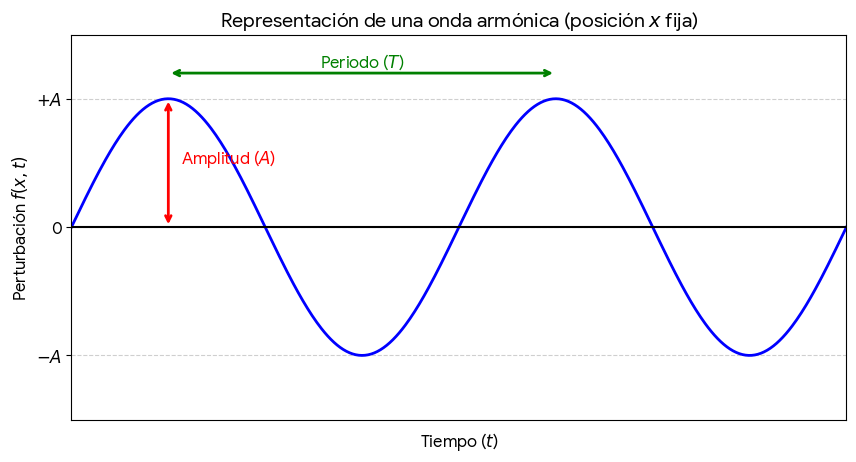
\includegraphics[width=13cm]{imagenes/1a.png}
					\caption{Evolución de una onda armónica en función del periodo T en un punto $x$ determinado}
				\end{figure}

				\vspace{1cm}

				\begin{figure}[H]
					\centering
					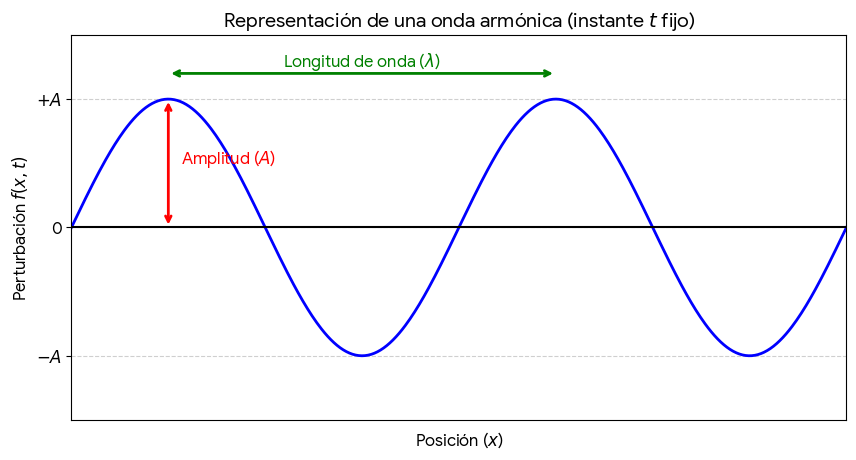
\includegraphics[width=13cm]{imagenes/1a-lambda.png}
					\caption{Evolución de una onda armónica en función de la longitud de onda $\lambda$ en un periodo de tiempo $T$ determinado}
				\end{figure}
			}

		\vspace{0.5cm}

		\item Calculad el valor númerico del número de onda $k$ y de la frecuencia angular $\omega$ de esta onda. A continuación, escribid la expresión de $E(x,t)$ sustituyendo los valores obtenidos (dejad $E_0$ y $\varphi$ como parámetros).

			{ \color{blue} 
				El objetivo es aplicar las fórmulas que relacionan la longitud de onda y la velocidad con el número de onda y la frecuencia angular, para finalmente construir la ecuación matemática de propagación en la dirección positiva del eje $x$.

				Para calcular el número de onda $k$, empleamos la relación descrita en la página 13, Fórmula [3]: $k = \frac{2\pi}{\lambda}$ [7]. 
				Sustituyendo el valor dado de $\lambda = 600 \text{ nm} = 600 \cdot 10^{-9} \text{ m}$ [8]:
				$$k = \frac{2\pi}{600 \cdot 10^{-9} \text{ m}} = \frac{\pi}{3 \cdot 10^{-7}} \approx 1,047 \cdot 10^7 \text{ m}^{-1}$$

				Para calcular la frecuencia angular $\omega$, utilizamos la relación de la velocidad de propagación de la página 14, Fórmula [9]: $v = \frac{\omega}{k}$, de la cual despejamos $\omega = v \cdot k$.
				Sustituyendo los datos del enunciado y el valor obtenido de $k$:
				$$\omega = (3 \cdot 10^8 \text{ m/s}) \cdot \left(\frac{\pi}{3 \cdot 10^{-7}} \text{ m}^{-1}\right) = \pi \cdot 10^{15} \approx 3,1415 \cdot 10^{15} \text{ rad/s}$$

				Al indicarnos que la onda se propaga en la dirección positiva del eje $x$, el argumento de la fase toma la forma $(kx - \omega t)$ según la Fórmula [1]. Sustituyendo los valores, la expresión queda:
				$$E(x,t) = E_0 \sin \left(1,047 \cdot 10^7 x - 3,1415 \cdot 10^{15} t + \varphi\right)$$
			}

		\item ¿Qué sucede con la velocidad de esta onda cuando se refracta del aire al agua ($n_{\text{agua}} = 1,33$)? ¿Aumenta, disminuye o se mantiene constante? Razonad la respuesta en función del índice de refracción.

			{ \color{blue} 
				La característica óptica fundamental de cualquier medio transparente se basa en su índice de refracción, el cual está definido en la página 22, Fórmula [10] como: $n = \frac{v_0}{v}$. En esta ecuación, $v_0$ representa la velocidad de propagación de la luz en el vacío y $v$ es la velocidad de propagación en el medio analizado.

				Despejando la velocidad $v$, llegamos a la expresión $v = \frac{v_0}{n}$. 

				La fórmula evidencia que la velocidad de propagación $v$ es inversamente proporcional al índice de refracción del medio $n$. La onda inicialmente se propaga por el aire, cuyo índice es muy próximo al del vacío ($n_1 = 1$), y posteriormente penetra en el agua, que posee un índice de refracción mayor ($n_{\text{agua}} = 1,33$). Como el denominador $n$ en la expresión de la velocidad aumenta, el cociente global se hace más pequeño.

				Por tanto, la velocidad de propagación de la onda \textbf{disminuye} al pasar del aire al agua.
			}
		\end{enumerate}
	\end{problem}

	% --- Exercise 2 ---
	\begin{problem}[Cuestión 2]
		Un haz de luz blanca incide desde el aire sobre una superficie plana de vidrio flint con un ángulo de incidencia de $\theta_1 = 43,2^\circ$ (medido respecto de la normal). Debido a la dispersión del vidrio, el índice de refracción depende de la longitud de onda. Suponed:

		\begin{equation}
			n_{\text{aire}} = 1 \qquad n_{\text{rojo}}=1,615 \qquad n_{\text{violeta}} = 1,655
		\end{equation}

		\begin{enumerate}[label=\alph*)]
			\item Calculad el ángulo de refracción dentro del vidrio para la componente roja (660 nm) y para la componente violeta (410 nm).

				{ \color{blue} 
					Se pide utilizar la ley fundamental de la refracción para encontrar el ángulo con el que cada color (longitud de onda) se desvía al penetrar en el vidrio. Como el índice de refracción varía según el color, calcularemos de forma independiente el ángulo de refracción para la componente roja y para la violeta.

					Para calcular los ángulos de refracción empleamos la \textbf{ley de Snell}, que está definida en la página 24, Fórmula [12]: $n_1 \sin \theta_1 = n_2 \sin \theta_2$. Como podemos ver, esta ley establece la relación entre los ángulos de incidencia y refracción y los índices de los medios 

					El hecho de que tengamos diferentes índices de refracción para diferentes longitudes de onda se debe al fenómeno de la \textbf{dispersión}, el cual se explica en la página 32.

					Sabiendo que el rayo incide desde el aire ($n_1 = 1$) con un ángulo $\theta_1 = 43,2^\circ$, despejamos el ángulo de refracción $\theta_2$ para cada color:
					$\theta_2 = \arcsin \left( \frac{n_1 \sin \theta_1}{n_2} \right)$

					\begin{enumerate}
						\item Para la componente roja ($n_{\text{rojo}} = 1,615$):          

						$$
						\theta_{2,\text{rojo}} = \arcsin \left( \frac{1 \cdot \sin(43,2^\circ)}{1,615} \right) = \arcsin \left( \frac{0,6845}{1,615} \right) = \arcsin (0,4238) \approx 25,08^\circ
						$$

						\vspace{0.5cm}

						\item Para la componente violeta ($n_{\text{violeta}} = 1,655$):

						$$
						\theta_{2,\text{violeta}} = \arcsin \left( \frac{1 \cdot \sin(43,2^\circ)}{1,655} \right) = \arcsin \left( \frac{0,6845}{1,655} \right) = \arcsin(0,4136) \approx 24,43^\circ
						$$
					\end{enumerate}
				}

			\item Dibujad el trazado de rayos de la cuestión.

				{ \color{blue} 
					La Figura 12 de la página 32 ilustra cómo, debido a que el índice de refracción es diferente para cada longitud de onda, las diferentes componentes de la luz se refractan con ángulos distintos. Por lo tanto, podemos tomarla como modelo para dibujar el trazado de rayos de la cuestión:

					\begin{figure}[H]
						\centering
						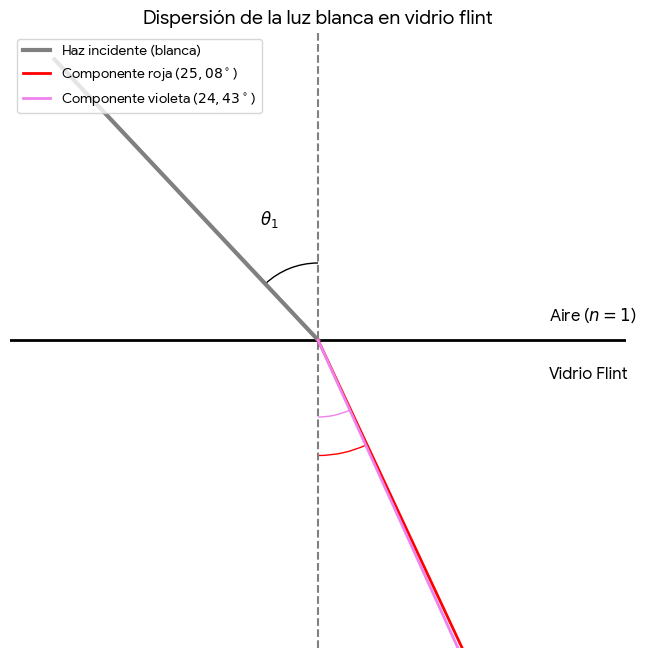
\includegraphics[width=10cm]{imagenes/2b.png}
						\caption{Trazado de rayos de la cuestión}
					\end{figure} 
				}

			\item Ahora considerad la interfaz vidrio-aire (el rayo se encuentra dentro del vidrio y llega a la superficie para salir al aire). Calculad el ángulo crítico $\theta_c$ para el rojo y para el violeta.

				{ \color{blue} 
					En esta situación opuesta, la luz viaja desde un medio más denso (el vidrio) hacia uno menos denso (el aire). El objetivo es encontrar el ángulo crítico a partir del cual ya no se produce refracción sino una reflexión interna total para cada una de las longitudes de onda.

					La condición a partir de la cual toda la luz se refleja y no hay refracción se describe en el Apartado 2.4 (páginas 26 y 27). La fórmula para hallar este ángulo límite se detalla en la página 27, Fórmula [18]: $\theta_{\text{crítico}} = \arcsin \left( \frac{n_2}{n_1} \right)$. 

					En este caso, el medio de origen es el vidrio ($n_1 = n_{\text{rojo}}$ o $n_{\text{violeta}}$) y el medio de destino es el aire ($n_2 = 1$). Por tanto, la ecuación que aplicamos es $\theta_c = \arcsin \left(\frac{1}{n_{\text{vidrio}}}\right)$.

					\begin{enumerate}
						\item Ángulo crítico para el rojo ($n_{\text{rojo}} = 1,615$):          

						$$
						\theta_{c,\text{rojo}} = \arcsin \left( \frac{1}{1,615} \right) = \arcsin(0,6192) \approx 38,26^\circ
						$$

						\vspace{0.5cm}

						\item Ángulo crítico para el violeta ($n_{\text{violeta}} = 1,655$):

						$$
						\theta_{c,\text{violeta}} = \arcsin \left( \frac{1}{1,655} \right) = \arcsin(0,6042) \approx 37,17^\circ
						$$
					\end{enumerate}

					A partir de estos ángulos, cualquier incidencia superior provocará la reflexión total del rayo correspondiente dentro del vidrio.
				}
		\end{enumerate}
	\end{problem}

	% --- Exercise 3 ---

	\begin{problem}[Cuestión 3]
	Indicad si las siguientes afirmaciones sobre ópticas son verdaderas (V) o falsas (F), justificando la respuesta con argumentos físicos y, si procede, con cálculos.

	\begin{enumerate}[label=\alph*)] 
		\item En una fibra óptica, la luz se guía por el núcleo porque su índice de refracción es mayor que el del revestimiento, lo que permite que se produzca reflexión interna total.

			{ \color{blue} 
				La afirmación es \textbf{verdadera} (V). Según se explica en el Apartado 2.5 (página 28), una fibra óptica está formada por un núcleo transparente rodeado por un revestimiento que posee un índice de refracción inferior al del núcleo. Esta característica permite que, si un haz de luz entra en la fibra, los rayos que se encuentran en un ángulo superior al llamado ángulo crítico respecto a las paredes sufran una reflexión interna total y queden confinados en su interior. Matemáticamente, el ángulo crítico se define en la página 27, mediante la Fórmula [18], como $\theta_c = \arcsin(\frac{n_2}{n_1})$. Para que el cálculo del arcoseno sea posible (y por tanto exista reflexión interna total), es estrictamente necesario que el índice de refracción del medio de destino ($n_2$) sea menor que el índice del medio original donde está viajando la luz ($n_1$).
			}

		\item Si aumenta el índice de refracción del revestimiento de una fibra óptica manteniendo constante el índice del núcleo, el ángulo crítico aumenta y la fibra puede aceptar un número mayor de rayos incidentes.

			{ \color{blue} 
				La afirmación es \textbf{falsa} (F). Es cierto que el ángulo crítico aumentaría, ya que, adaptado a la nomenclatura de fibras, este ángulo se calcula mediante la Fórmula [20] de la página 29: $\theta_c = \arcsin(n_3/n_2)$. Si el índice del revestimiento ($n_3$) aumenta, el cociente $n_3/n_2$ es mayor y su arcoseno crece. 

				Sin embargo, esta variación perjudica la capacidad de la fibra para captar luz. El ángulo de aceptación máximo de la fibra ($\theta_1$) se halla mediante la expresión de la apertura numérica, detallada en la página 31, Fórmula [31]: $\sin \theta_1 = \sqrt{\left (\frac{n_2}{n_1} \right)^2 - \left(\frac{n_3}{n_1} \right)^2}$. Si el valor de $n_3$ aumenta, el sustraendo dentro de la raíz cuadrada se hace más grande, lo que resulta en un seno de apertura menor. En consecuencia, el ángulo $\theta_1$ disminuye, lo que provoca que el cono de aceptación se reduzca y la fibra acepte un \textbf{menor} número de rayos incidentes, no mayor.
			}

		\item Una fibra óptica con índices $n_{\text{núcleo}} = 1,62$ y $n_{\text{revestimiento}} = 1,56$, inmersa en aire ($n_{\text{ext}} = 1$), tiene un ángulo máximo de aceptación aproximadamente igual a $\theta_{\text{max}} \approx 32^\circ$.

			{ \color{blue} 
				La afirmación es \text{falsa} (F). En el caso concreto en el que el medio exterior es el aire ($n_1 = 1$), el ángulo de aceptación $\theta_1$ se evalúa de manera simplificada con la Fórmula [32] de la página 31: $\sin\theta_1 = \sqrt{n_2^2 - n_3^2}$. 

				Sustituyendo los datos del problema, donde $n_2 = 1,62$ y $n_3 = 1,56$, el cálculo se desarrolla así:

				$$
				\sin \theta_1 = \sqrt{1,62^2 - 1,56^2} = \sqrt{2,6244 - 2,4336} = \sqrt{0,1908} \approx 0,4368
				$$

				A continuación, despejamos el ángulo resolviendo el arcoseno de este valor:

				$$
				\theta_1 = \arcsin(0,4368) \approx 25,89^\circ
				$$

				Como queda demostrado matemáticamente, el ángulo máximo de aceptación se sitúa en torno a los $25,9^\circ$ y no alcanza los $32^\circ$ que postula la afirmación.
			}
		\end{enumerate}
	\end{problem}

	% --- Exercise 4 ---
	\begin{problem}[Cuestión 4]
	Dos ondas electromagnéticas monocromáticas, con intensidades $I_1$ e $I_2$, se propagan por un mismo medio e interfieren en un punto del espacio. La intensidad de la primera onda es $I_1 = 2 \text{W/m}^2$, mientras que la intensidad de la segunda onda es desconocida.

	Variando la diferencia de fase entre dos ondas se observa que la intensidad resultante puede alcanzar un valor máximo de

	\begin{equation}
		I_{\text{max}} = 18 W/m^2
	\end{equation}

	\vspace{0.25cm}

	y un valor mínimo de

	\begin{equation}
		I_{\text{min}} = 2 W/m^2
	\end{equation}

	\vspace{0.25cm}

	Determinad la intensidad de la segunda onda $I_2$.

	\vspace{0.5cm}

	{ \color{blue} 
		El problema nos pide determinar la intensidad de una onda desconocida a partir de los valores extremos que se producen al interferir con otra onda de intensidad conocida.

		Cuando dos ondas se superponen, la intensidad resultante no es simplemente la suma aritmética de sus intensidades, sino que incluye un término adicional de interferencia que depende directamente de la diferencia de fase temporal y espacial entre ellas. La expresión matemática general para esta intensidad se detalla en la página 43, Fórmula [61]: $I = I_1 + I_2 + 2 \sqrt{I_1 I_2} \cos {\delta}$.

		La intensidad resultante alcanza su valor máximo, lo que produce lo que conocemos como interferencia constructiva, cuando las ondas están en fase y el coseno alcanza su valor máximo de 1. Esta relación particular se encuentra explícita en la página 43, Fórmula [62]: $I_{\text{max}} = I_1 + I_2 + 2 \sqrt{I_1 I_2}$.

		Contrario a esto, los mínimos de intensidad se obtienen mediante interferencia destructiva, lo cual ocurre cuando el desfase hace que el coseno valga -1. Esta ecuación se define de forma análoga en la página 44, Fórmula [63]: $I_{\text{min} = I_1 + I_2 - 2 \sqrt{I_1 I_2}}$:

		Para hallar $I_2$, podemos aprovecharnos de las fórmulas [62] y [63]. Un modo muy sencillo de despejar la incógnita es sumar ambas expresiones matemáticas, de modo que el término que contiene la raíz cuadrada se anulará:

		$$
		I_{\text{max}} + I_{\text{min}} = \left(I_1 + I_2 + 2 \sqrt{I_1 I_2} \right) + \left( I_1 + I_2 - 2 \sqrt{I_1 I_2} \right)
		$$

		$$
		I_{\text{max}} + I_{\text{min}} = 2(I_1 + I_2)
		$$

		A continuación, sustituimos los valores numéricos proporcionados en el enunciado del problema:

		$$
		18 + 2 = 2(2 + I_2)
		$$
		$$
		20 = 4 + 2 I_2
		$$
		$$
		16 = 2 I_2
		$$
		$$
		I_2 = 8 \text{ W/m}^2
		$$

		A modo de comprobación, podemos introducir el valor obtenido $I_2  =8$ en la fórmula de la intensidad mínima [63] para verificar la consistencia matemática: 

		$$
		I_{\text{min}} = 2 + 8 - 2 \sqrt{2 \cdot 8} = 10 - 2 \sqrt{16} = 10 - 8 = 2 \text{W/m}^2
		$$

		Dado que el valor coincide con los datos originales, queda confirmado que la intensidad de la segunda onda es de
	}
	\end{problem}

	% --- Exercise 5 ---
	\begin{problem}[Cuestión 5]
		Entrad en el siguiente enlace (https://www.geogebra.org/m/ZSbeWGbe) donde encontraréis un simulador del experimento de la doble rendija de Young. Contestad a las siguientes preguntas utilizando el simulador y adjuntad capturas de pantalla en las que se muestre lo que habéis hecho para poder responderlas. 

		\begin{enumerate}[label=\alph*)]
			\item Cuando entráis en el simulador, se puede seleccionar que muestre la interferencia, la difracción o ambas. Mostrad cómo queda cada una de estas configuraciones y explicad cómo están relacionadas.

				{ \color{blue} 
					\begin{itemize}
						\item \textbf{Solo interferencia}: Al marcar esta opción, el simulador dibuja una serie continua de máximos y mínimos que tienen exactamente la misma amplitud y están espaciados de manera totalmente uniforme. Este gráfico representa el patrón ideal de interferencia de la doble rendija, asumiendo teóricamente que las rendijas son fuentes puntuales. Matemáticamente, este patrón surge porque la diferencia de caminos de la luz crea interferencias constructivas. La posición angular de estos máximos viene dada por la página 50, fórmula [80]: $d \sin \theta= m \lambda$, y la posición en la pantalla por la fórmula [85]: $y=m \frac{\lambda L}{d}$

						\begin{figure}[H]
							\centering
							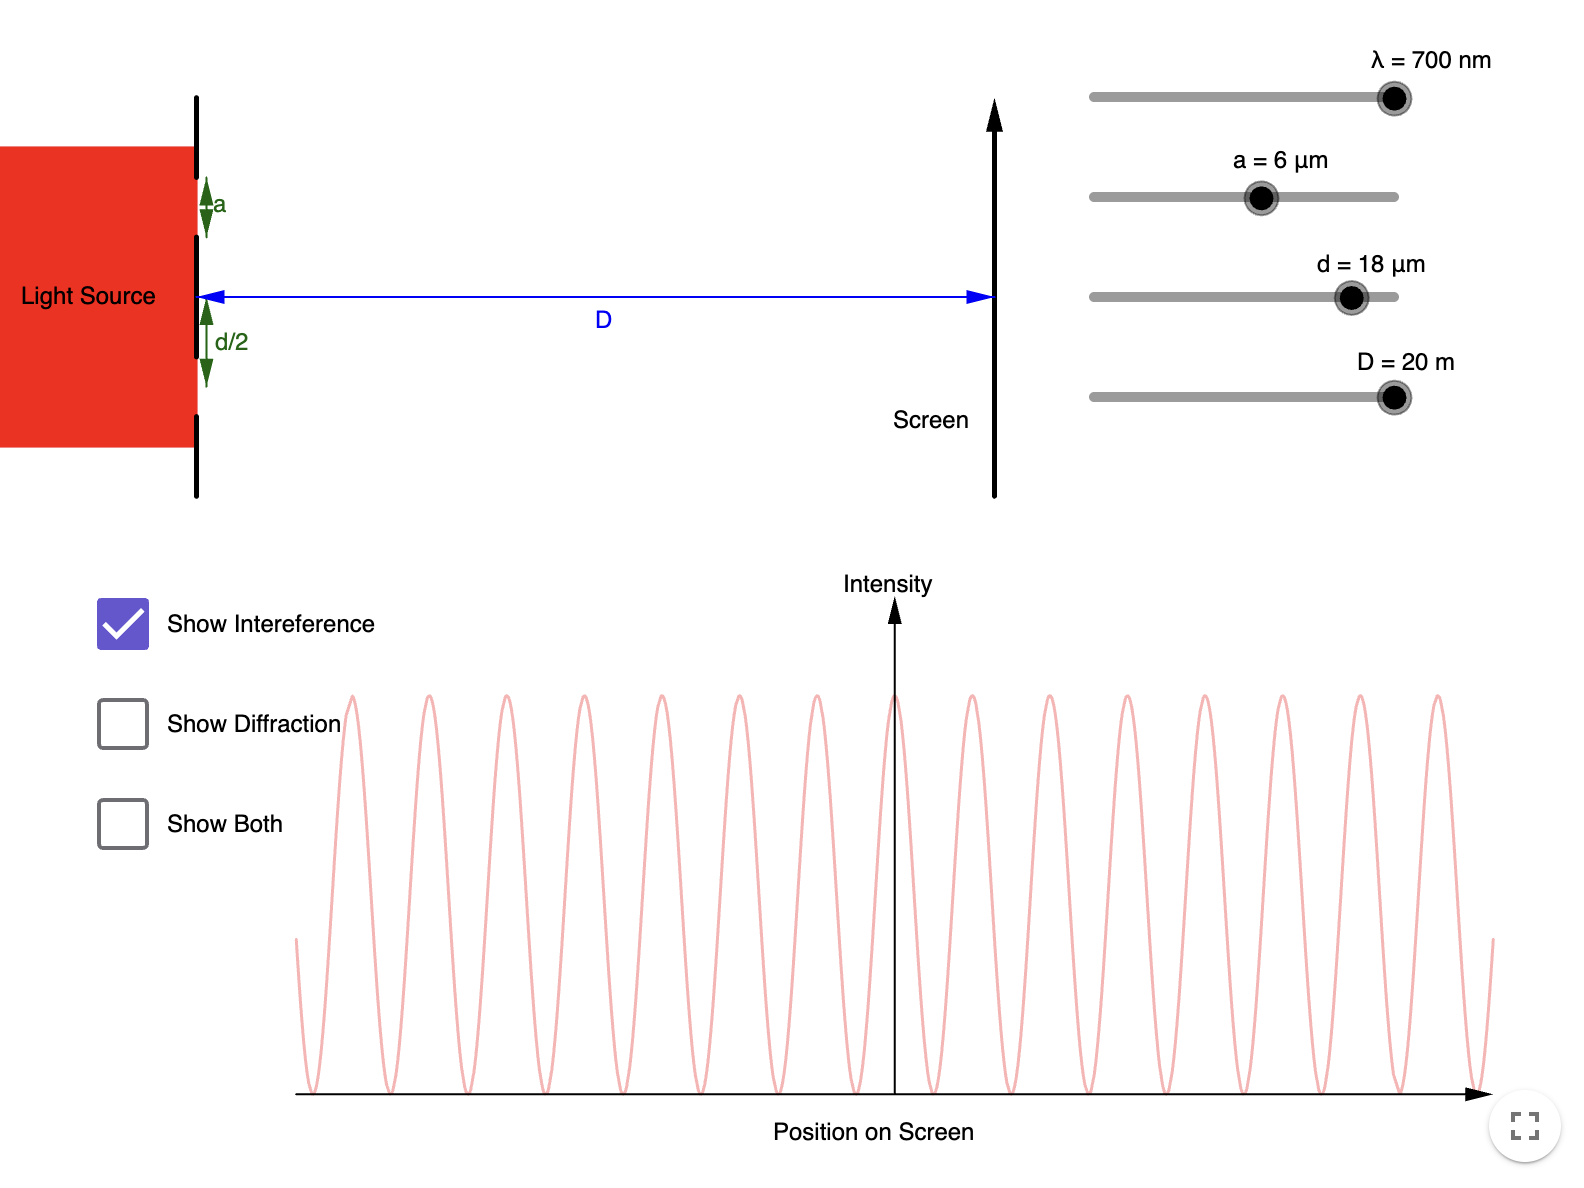
\includegraphics[width=13cm]{imagenes/5a-interferencia.png}
							\caption{Configuración de solo interferencia}
						\end{figure}

						\vspace{0.5cm}

						\item \textbf{Solo difracción}: La pantalla muestra una curva en forma de campana ancha con pequeñas ondulaciones a los lados cuya intensidad decae rápidamente a medida que nos alejamos del centro. Este gráfico muestra el patrón de difracción generado por una sola rendija debido a su anchura física a. La condición para encontrar los mínimos de intensidad en este patrón individual está explicada en la página 53, fórmula [87]: $a \sin \theta = m \lambda$.

						\begin{figure}[H]
							\centering
							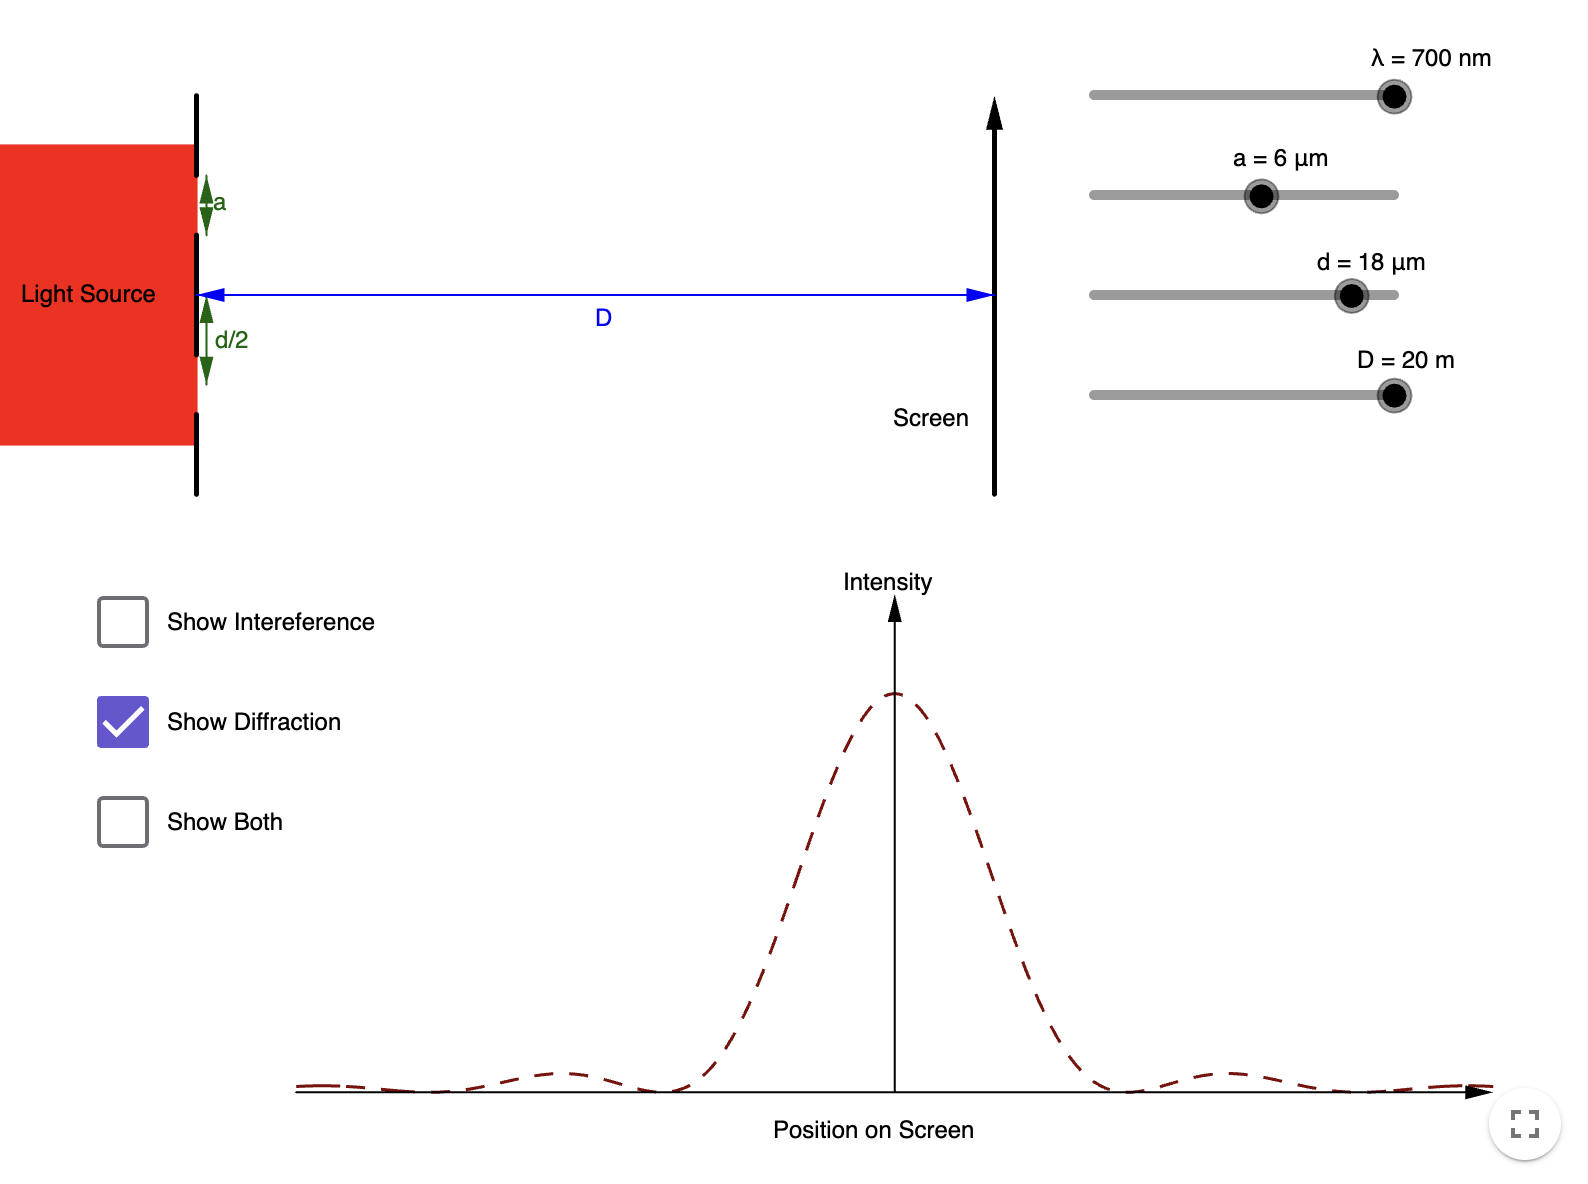
\includegraphics[width=13cm]{imagenes/5a-difraccion.png}
							\caption{Configuración de solo difracción}
						\end{figure}

						\item \textbf{Mostrar ambos}: Al marcar ambas, el simulador muestra el patrón real que observaríamos en el laboratorio: franjas de interferencia estrechas cuya altura ya no es constante, sino que están delimitadas por una línea de puntos que coincide exactamente con la curva de difracción del caso anterior.

						\begin{figure}[H]
							\centering
							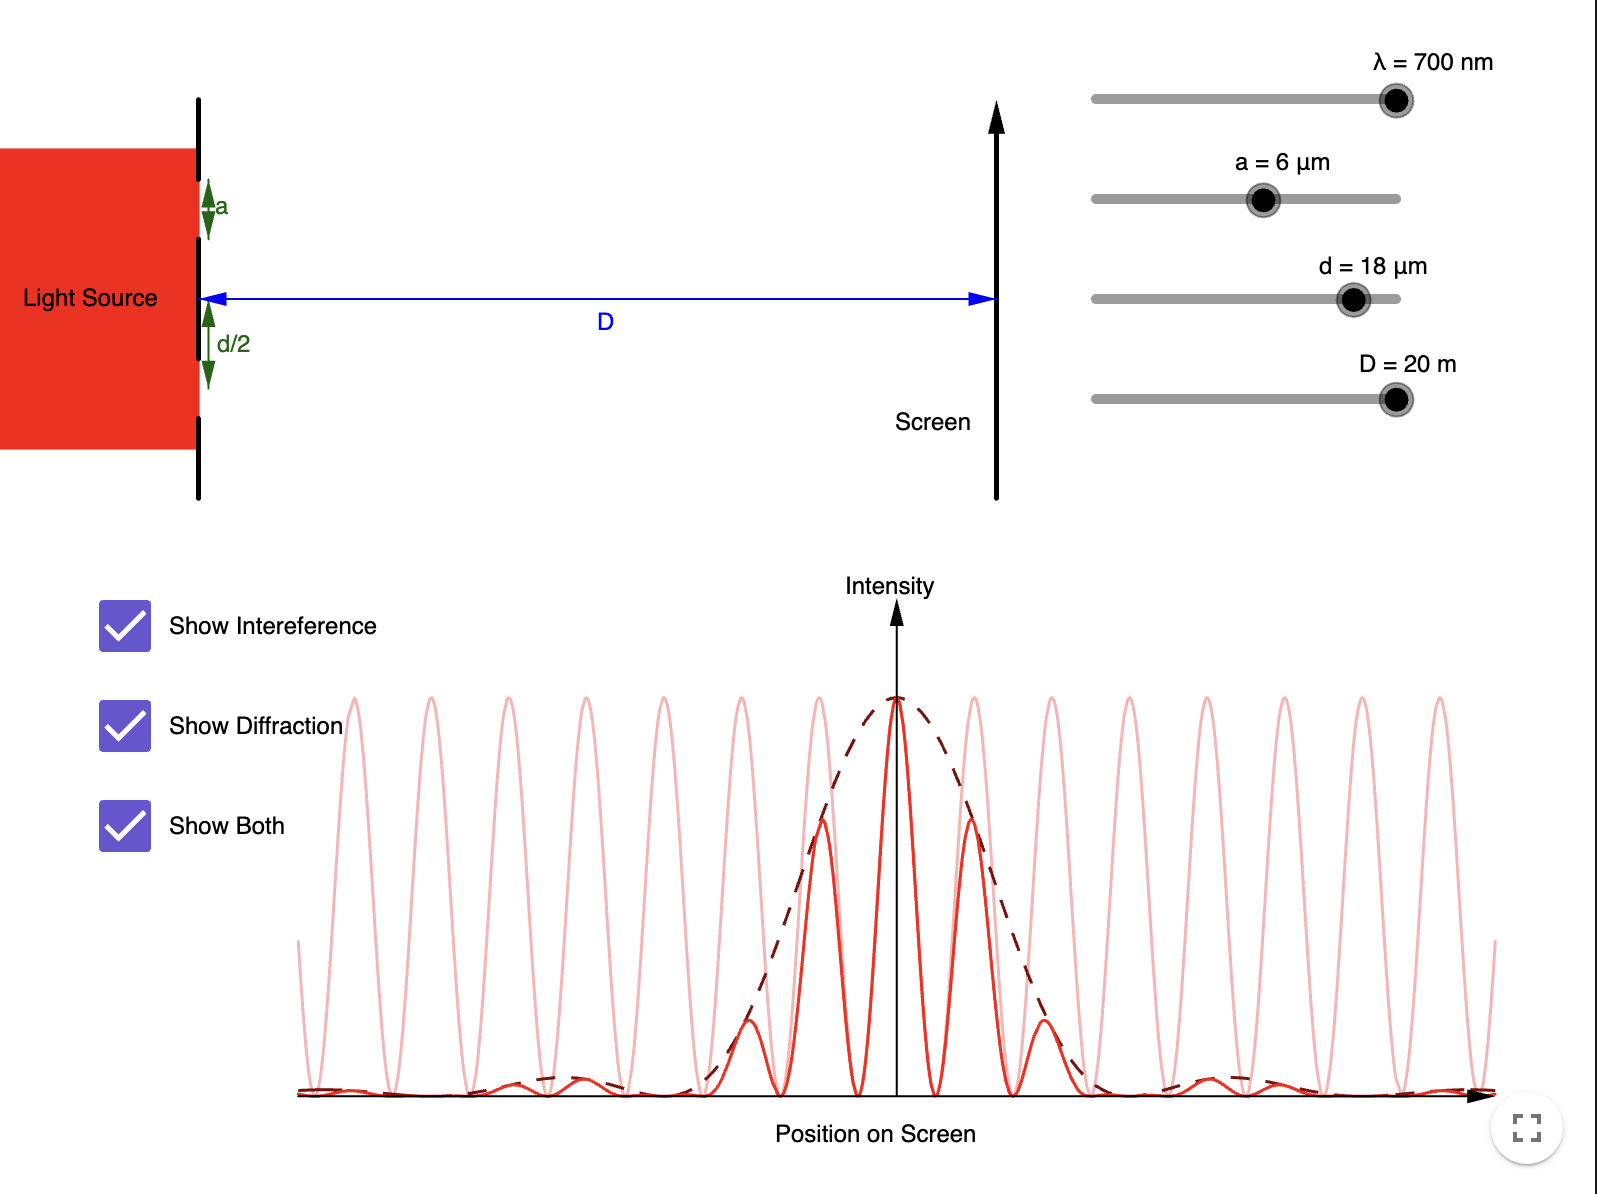
\includegraphics[width=13cm]{imagenes/5a-both.png}
							\caption{Configuración de ambas opciones combinadas}
						\end{figure}
					\end{itemize}

					La física subyacente que relaciona estas configuraciones se explica detalladamente en las páginas 53 y 54 de los apuntes. En el experimento real de Young, cada una de las dos rendijas no es un punto ideal, sino que tiene una anchura $a$. Por lo tanto, la luz se difracta primero al pasar por cada rendija individual (el frente de onda se "abre"), lo que crea una envolvente de intensidades dictada por la difracción. Tras ello, las ondas difractadas provenientes de la primera rendija se superponen en el espacio con las de la segunda rendija, dando lugar al fenómeno de la interferencia.

					En definitiva, el patrón observable es producto de ambos efectos. Por un lado, la difracción actúa como una envolvente que modula y limita cuánta luz puede llegar a cada zona de la pantalla, mientras que por otra, la interferencia aporta la "estructura fina" que oscila dentro de esa envolvente. Dado que la anchura de la rendija $a$ suele ser menor que la separación $d$, el patrón de difracción es mucho más ancho que el espaciado de interferencia. Esto obedece a la ley fundamental detallada en la página 55: "las distancias características del elemento difractor son inversamente proporcionales al espaciado de los máximos".
				}

			\vspace{0.5cm}

			\item ¿De qué parámetro es independiente el patrón de interferencia? Fijaos en que solo tenéis que tener seleccionado el patrón de interferencia.

				{ \color{blue} 
					Si interactuamos con el simulador teniendo seleccionada solo la opción "Show Interference" , apreciamos que el gráfico muestra una serie continua de picos de amplitud idéntica. La posición y separación de estos máximos de interferencia depende exclusivamente de la longitud de onda ($\lambda$), la separación entre las rendijas ($d$) y la distancia hasta la pantalla ($D$ o $L$ en los apuntes), tal como describe la fórmula matemática $y=m \frac{\lambda L}{d}$.

					La anchura de la rendija ($a$) es el parámetro responsable de dictar el patrón de difracción. Determina la posición de sus mínimos mediante la relación $a \sin \theta=m \lambda$. Al visualizar solo la interferencia, el simulador asume teóricamente que las rendijas son fuentes puntuales infinitamente estrechas, por lo que el parámetro $a$ no altera la gráfica obtenida. La difracción producida por la anchura de la rendija $a$ actúa como una envolvente global que modula y recorta la intensidad de los picos de interferencia si se activan ambos fenómenos a la vez ("Show Both").

					Por tanto, el patrón de interferencia puro es independiente de la anchura de las rendijas ($a$).

					\begin{figure}[H]
						\centering
						\includegraphics[width=13cm]{imagenes/5b-a1ng}
						\caption{Solo interferencia con el valor $a = 1\; \mu \text{m}$}
					\end{figure}

					\vspace{1.75cm}

					\begin{figure}[H]
						\centering
						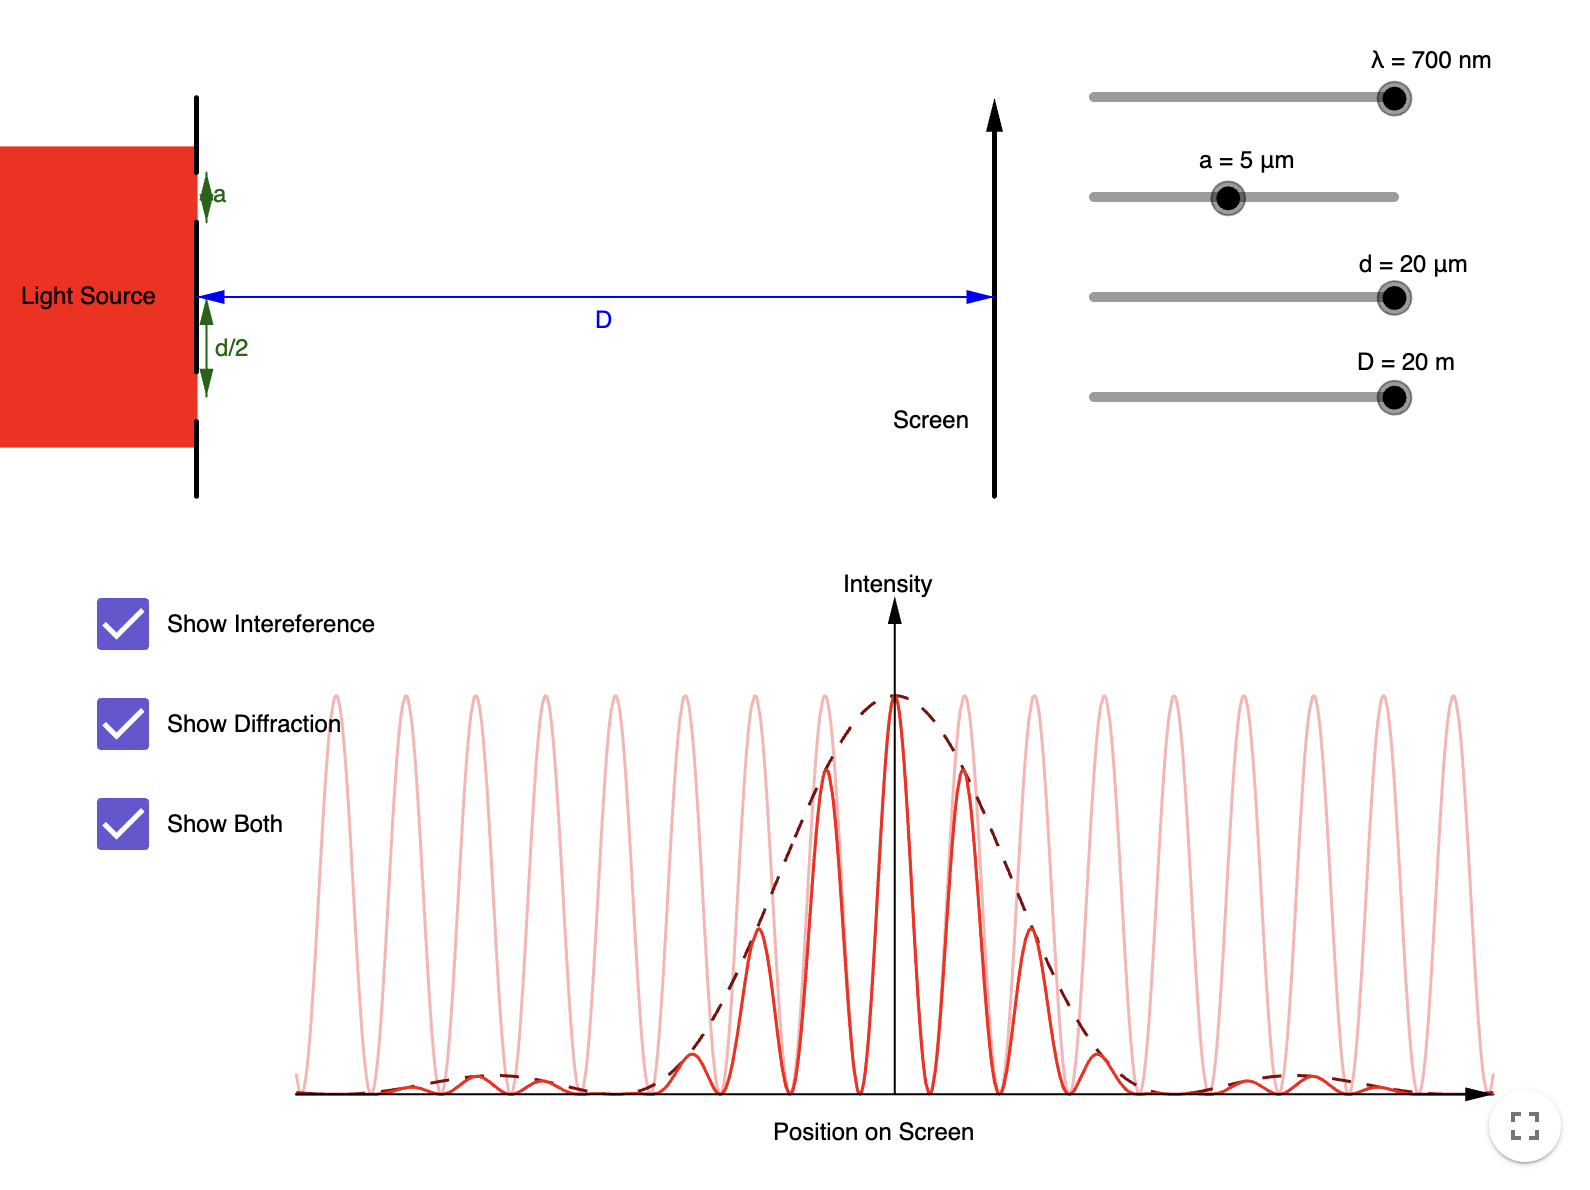
\includegraphics[width=13cm]{imagenes/5b-a5.png}
						\caption{Solo interferencia con el valor $a = 5 \; \mu \text{m}$}
					\end{figure}
				}

			\item Cuando la separación de la rendija ($d$) es cuatro veces mayor que la anchura de la rendija ($a$), ¿qué máximo de interferencia es el primero que falta? Fijaos en que en este caso tenéis que tener seleccionado el patrón de interferencia y el de difracción. Si no observáis que desaparece ninguno, modificad la longitud de onda $\lambda$ y la distancia $D$ hasta que lo observéis.

				{ \color{blue} 
					El fenómeno de los "máximos ausentes" ocurre cuando la posición angular de un \textbf{máximo de interferencia} coincide exactamente con la posición angular de un \textbf{mínimo de difracción}. La curva de difracción actúa como una envolvente global. Si esta envolvente llega a un valor de cero, cualquier pico de interferencia que se encuentre en esa posición exacta quedará anulado.

					Las posiciones angulares de los \textbf{máximos de interferencia} vienen dadas en la página 50, Fórmula [80]: $d \sin \theta = m \lambda$, donde $m$ es el orden del máximo de interferencia ($m = 0, 1, 2, 3, \dots$).

					Las posiciones angulares de los \textbf{mínimos de difracción} causados por una sola rendija se definen en la página 53, fórmula [87]: $a \text{ sen } \theta = n\lambda$, donde $n$ es el orden del mínimo de difracción ($n = 1, 2, 3, \dots$). 

					Para encontrar el punto donde coinciden, igualamos el término $\text{sen } \theta$ de ambas ecuaciones:

					$$\frac{m\lambda}{d} = \frac{n\lambda}{a}$$

					Simplificando la longitud de onda $\lambda$ de ambos lados, obtenemos la relación:

					$$m = n \left( \frac{d}{a} \right)$$

					Sabiendo por el enunciado que la separación $d$ es cuatro veces la anchura $a$ ($d = 4a$), sustituimos:

					$$m = n \left( \frac{4a}{a} \right) = 4n$$

					Para hallar el \textbf{primer} máximo de interferencia ausente, evaluamos la posición en la que cae el \textbf{primer} mínimo de difracción ($n = 1$):
					$$m = 4 \cdot 1 = 4$$

					Por lo tanto, queda demostrado que el \textbf{4º máximo de interferencia} coincide espacialmente con el 1º mínimo de difracción y desaparece.

					\begin{figure}[H]
						\centering
						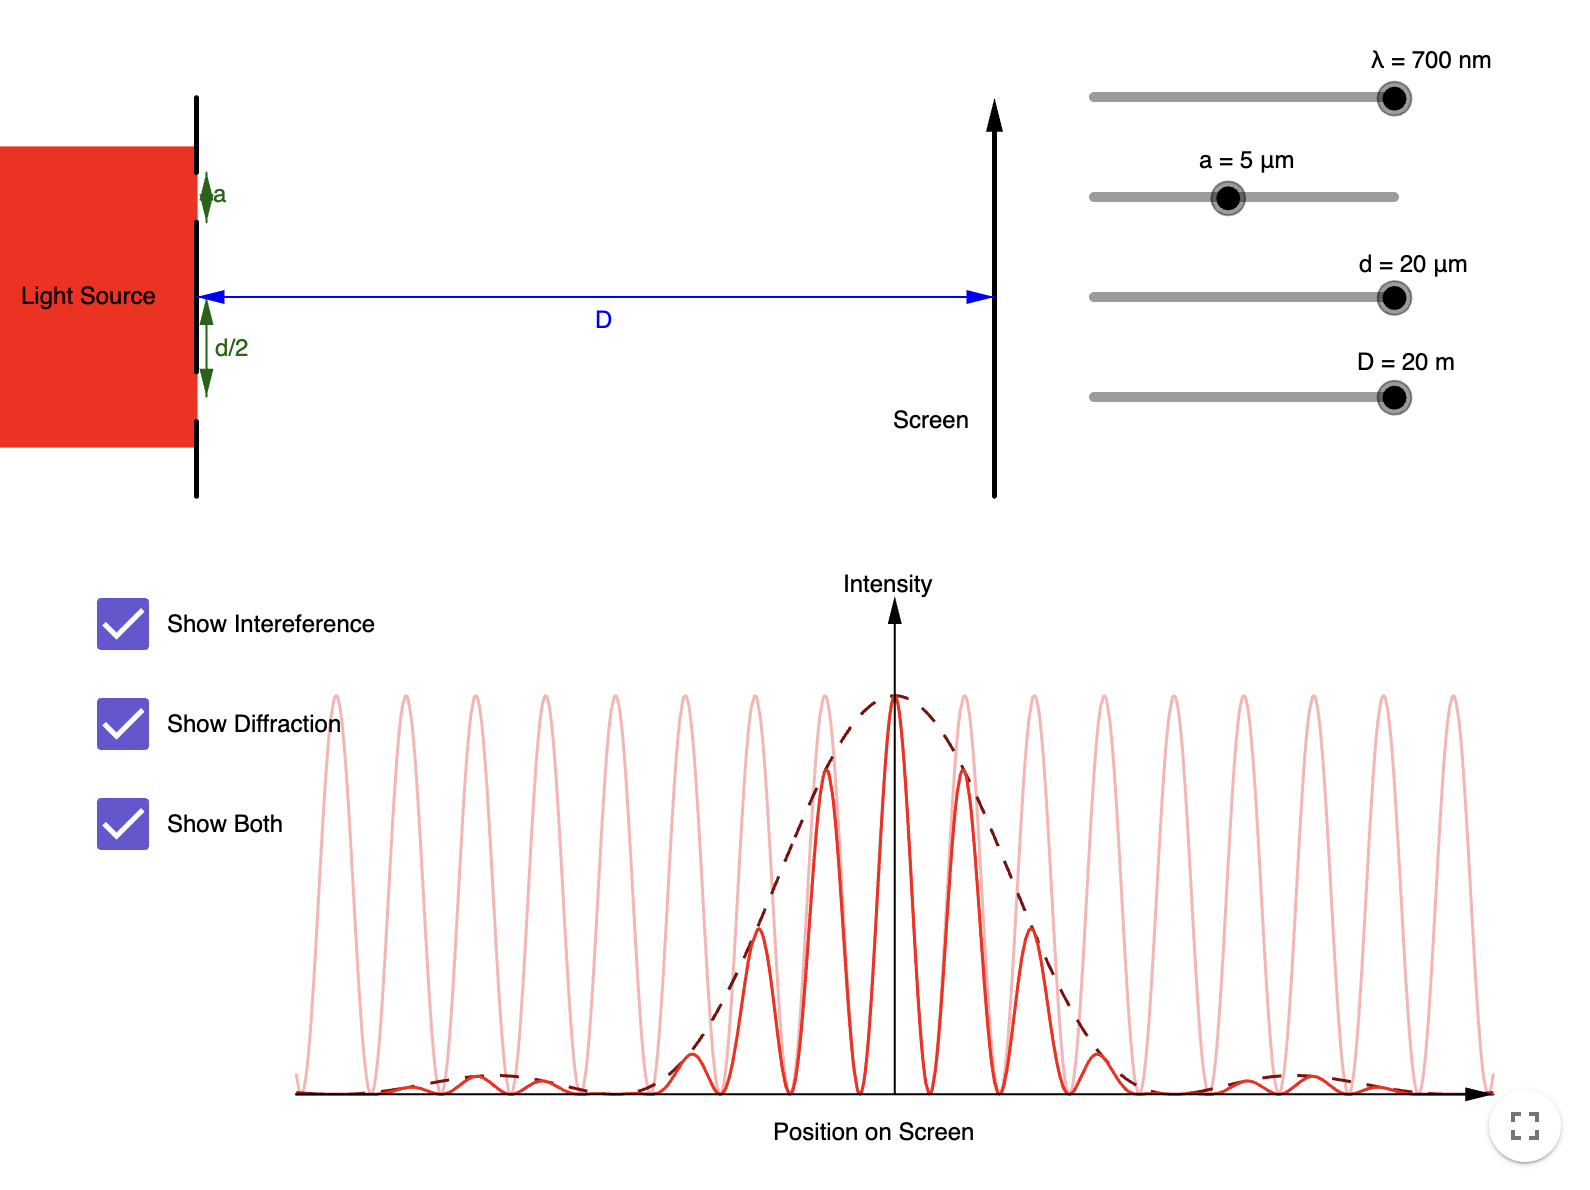
\includegraphics[width=13cm]{imagenes/5c.png}
						\caption{Mostrando ambas opciones con el valor $a = 4 \; \mu \text{m}$ y $d = 20 \; \text{m}$}
					\end{figure}
				}

			\item Determinad cuál es el efecto de variar la anchura de las rendijas, $a$, y si variando este parámetro los máximos seguirán coincidiendo en el espacio o no.

				{ \color{blue} 
					El efecto de variar la anchura de las rendijas, $a$, se consigue al modificar exclusivamente la \textbf{envolvente de difracción} global que modula la intensidad de la luz en la pantalla.

					Según la relación matemática para los mínimos de difracción de la página 53, Fórmula [87] ($a \sin \theta = n\lambda$), existe una proporcionalidad inversa. Esto significa que si \textbf{aumentamos la anchura $a$}, la campana o envolvente de difracción se hará \textbf{más estrecha}. Por el contrario, si \textbf{disminuimos $a$}, la envolvente de difracción se "abrirá" y se hará mucho \textbf{más ancha}.

					Los máximos de interferencia seguirán coincidiendo en el espacio, ya que las posiciones espaciales exactas de los picos de interferencia no cambian en absoluto. La ubicación de los máximos de interferencia depende únicamente de la separación entre las dos rendijas ($d$) y de la longitud de onda de la luz ($\lambda$), lo cual se rige por la ecuación de la página 50, fórmula [80] ($d \text{ sen } \theta = m\lambda$). 

					Como el parámetro $d$ no varía, las franjas de interferencia (los picos estrechos) seguirán apareciendo exactamente en las mismas posiciones espaciales sobre la pantalla. Lo único que cambia al alterar el valor de $a$ es la \textbf{intensidad lumínica} con la que brillan esos máximos y cuáles de ellos desaparecen visualmente, puesto que los mínimos de difracción se habrán desplazado a nuevas zonas.

					\begin{figure}[H]
						\centering
						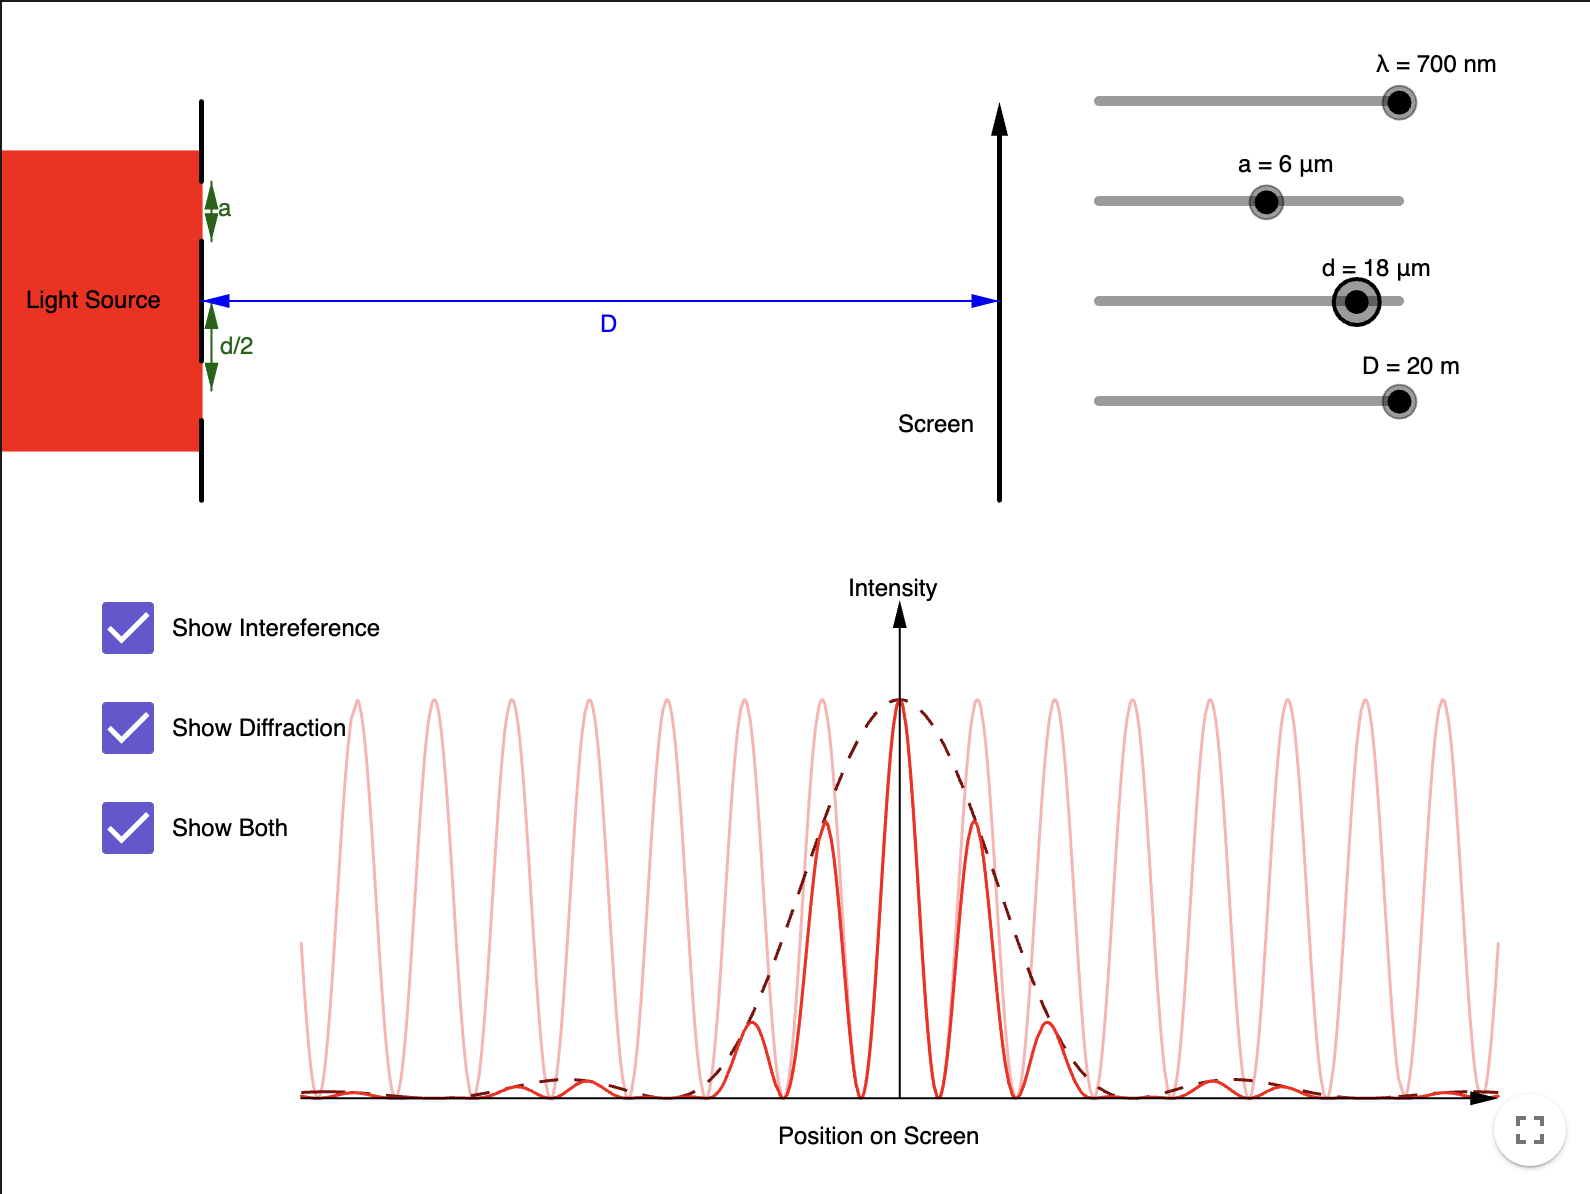
\includegraphics[width=13cm]{imagenes/5d-rendija-ancha.png}
						\caption{Rendija ancha con el valor $a = 6 \; \mu \text{m}$ y $d = 3a \; \text{m}$}
					\end{figure}

					\vspace{1cm}

					\begin{figure}[H]
						\centering
						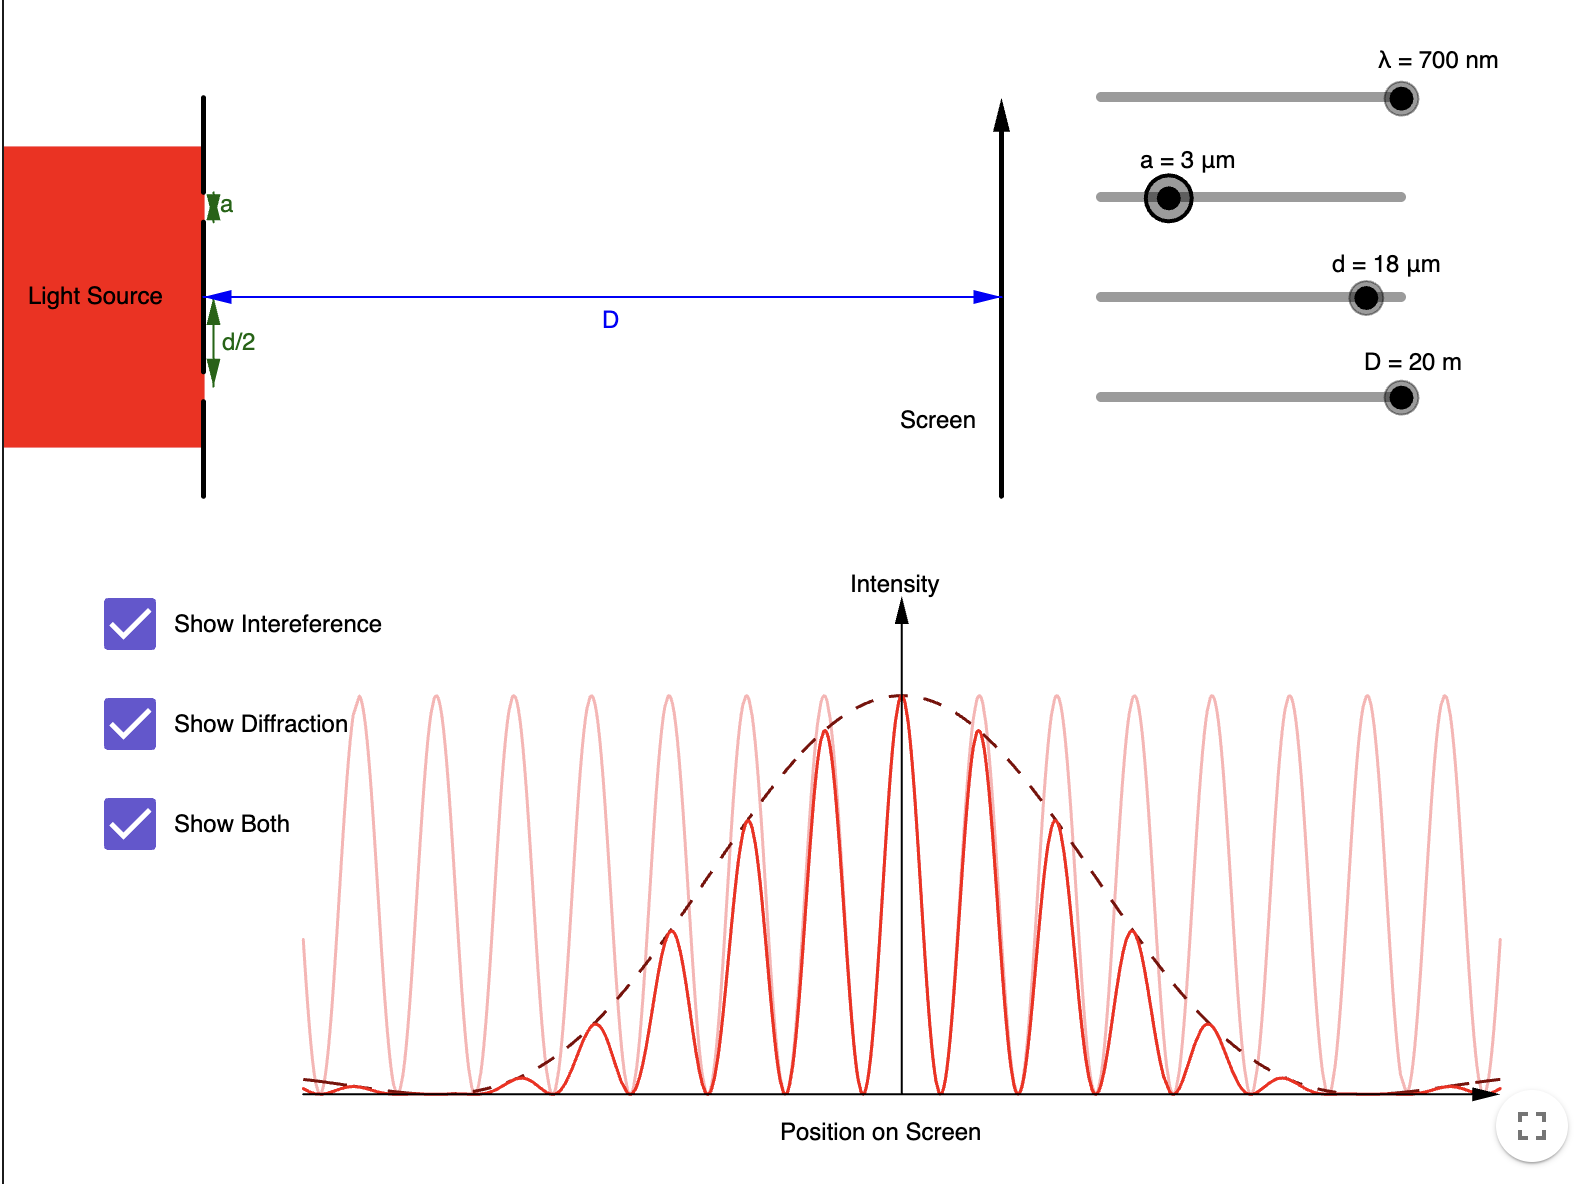
\includegraphics[width=13cm]{imagenes/5d-rendija-estrecha.png}
						\caption{Rendija estrecha con el valor $a = 3 \; \mu \text{m}$ y $d = 6a \; \text{m}$}
					\end{figure}
				}
		\end{enumerate}
	\end{problem}

	% --- Exercise 6 ---
	\begin{problem}[Cuestión 6]
		Un átomo presenta dos niveles de energía $E_1$ y $E_2$, con una separación energética:

		\begin{equation}
			\Delta E=E_2 - E_1 = 2,1 \; \text{eV}
		\end{equation}

		\vspace{0.25cm}

		\textbf{Datos}: $h=6,626 \times 10^{-34} \; J \cdot s, \quad c= 3 \times 10^8 m/s, \quad 1 \; \text{eV} = 1,602 \times 10^{-19} \; \text{J}$

		\begin{enumerate}[label=\alph*)]
			\item Calculad la frecuencia $f$ del fotón emitido en la transición $E_2 \to E_1$.

				{ \color{blue} 
					Para ello, primero convertiremos la diferencia de energía de electronvoltios (eV) a julios (J) y luego aplicaremos la relación fundamental de Planck que vincula la energía del fotón con su frecuencia.

					Según el principio de conservación de la energía y la descripción cuántica de la luz (descrito en el Apartado 4.5.3 referente a la emisión espontánea), la frecuencia $f$ de un fotón emitido en una transición entre dos niveles energéticos se obtiene a partir de la página 72, Fórmula [96]: $f = \frac{E_2 - E_1}{h}$. Esta ecuación se deriva directamente de la hipótesis de Einstein y de la ecuación de Planck detallada en la página 65, Fórmula [88]: $E = hf$ [2].

					Dada la justificación sobre cómo abordar este problema, pasamos a los cálculos. En primer lugar, convertimos la diferencia de energía a julios:

					$$
					\Delta E = 2,1 \text{ eV} \cdot \left( 1,602 \cdot 10^{-19} \text{ J/eV} \right) = 3,3642 \cdot 10^{-19} \text{ J}
					$$

					Sustituimos los valores en la fórmula de la frecuencia:

					$$
					f = \frac{\Delta E}{h} = \frac{3,3642 \cdot 10^{-19} \text{ J}}{6,626 \cdot 10^{-34} \text{ J}\cdot\text{s}} \approx 5,077 \cdot 10^{14} \text{ Hz}
					$$

					El fotón emitido tiene una frecuencia aproximada de $5,077 \cdot 10^{14} \text{ Hz}$.
				}

			\item Explicad por qué la luz producida por emisión espontánea, aun estando formada por fotones con la misma energía (y, por tanto, la misma frecuencia), no es luz coherente como la luz láser.

				{ \color{blue} 
					La condición de coherencia, definida en la página 47, implica que la diferencia de fase entre diversas ondas debe mantenerse constante a lo largo del tiempo. 

					En el proceso de \textbf{emisión espontánea}, explicado en las páginas 71 y 72, un electrón en un estado excitado cae espontáneamente a un nivel inferior emitiendo un fotón. Como se detalla en el paso 2 del funcionamiento del láser en la página 81, en este proceso los átomos "emiten fotones de cualquier fase y en cualquier dirección". Al ser emitidos de forma totalmente aleatoria e independiente por millones de átomos distintos, su diferencia de fase no conserva ninguna constancia, lo cual deriva en luz completamente incoherente [6].

					En contraposición, la luz láser se fundamenta en la \textbf{emisión estimulada} (página 70, Apartado 4.5.2). En este mecanismo, un fotón incidente fuerza al electrón a decaer emitiendo un nuevo fotón que es estrictamente idéntico al fotón incidente, con la misma frecuencia y fase, y misma dirección, tal y como se detalla en la página 82, paso 5). Esta igualdad de fase entre los fotones incidentes y emitidos es lo que dota a la luz láser de su característica coherencia.
				}
		\end{enumerate}
	\end{problem}

	% --- Problema ---
	\begin{problem}[Problema]
		Una fibra óptica está formada por un núcleo de índice de refracción $n_2=1,48$ y un revestimiento de índice $n_3=1,46$. La luz incide desde un medio exterior de índice $n_1$.

		\begin{enumerate}[label=\alph*)]
			\item Dibujad la fibra óptica del Problema indicando el recorrido de los rayos y los ángulos.

				\begin{figure}[H]
					\centering
					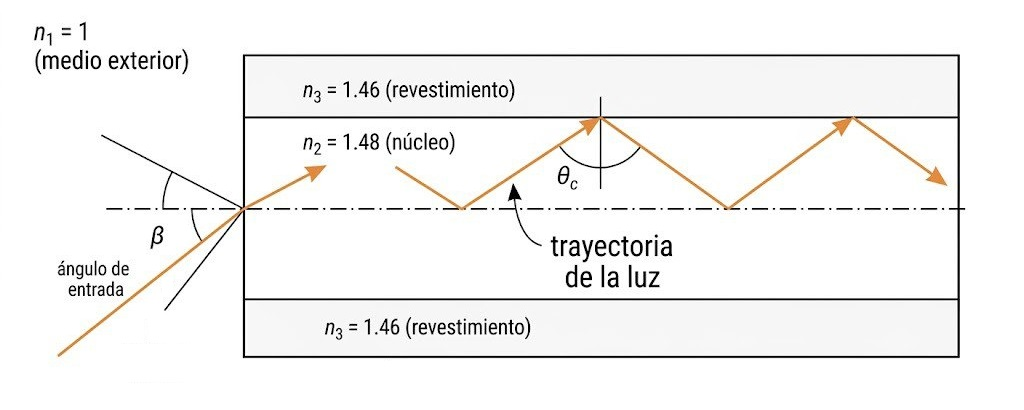
\includegraphics[width=13cm]{imagenes/problema.jpg}
					\caption{Representación gráfica de la fibra óptica a analizar}
				\end{figure}

			\item Para $n_1=1$ (aire), calculad el ángulo crítico en la frontera núcleo-revestimiento.

				{ \color{blue} 
					El ángulo crítico se calcula empleando la condición descrita en la página 29, Fórmula [20], la cual se deduce a partir de la ley de Snell para la reflexión total: $\theta_c = \arcsin\left(\frac{n_3}{n_2}\right)$ (en los apuntes aparece con la notación de $\theta_2$ o $\theta_c$ para ese ángulo interno).

					Dicho lo cual, pasamos a realizar el cálculo sustituyendo los índices de refracción del núcleo ($n_2 = 1,48$) y del revestimiento ($n_3 = 1,46$):
					$$\theta_c = \arcsin\left(\frac{1,46}{1,48}\right) = \arcsin(0,98648)$$
					$$\theta_c \approx 80,57^\circ$$

					El ángulo crítico en la frontera núcleo-revestimiento es de, aproximadamente, $\boxed{80,57^\circ}$.
				}

			\item Para $n_1=1$ (aire), determinad la mitad del ángulo del cono de aceptación $\theta_1$.

				{ \color{blue} 
					El objetivo de este apartado es hallar el ángulo de incidencia máximo desde el exterior que hace que la luz sufra reflexión total dentro de la fibra.

					Como el medio exterior es el aire ($n_1 = 1$), la fórmula que relaciona directamente este ángulo de aceptación con los índices internos de la fibra se encuentra simplificada en la página 31, Fórmula [32]: $\sin \theta_1 = \sqrt{n_2^2 - n_3^2}$.

					Ahora que tenemos la fórmula a aplicar identificada, sustituimos los valores numéricos:

					$$\sin \theta_1 = \sqrt{1,48^2 - 1,46^2} = \sqrt{2,1904 - 2,1316} = \sqrt{0,0588} \approx 0,2425$$

					A continuación, despejamos el ángulo resolviendo el arcoseno:

					$$\theta_1 = \arcsin(0,2425) \approx 14,04^\circ$$

					La mitad del ángulo del cono de aceptación es de aproximadamente $\boxed{14,04^\circ}$.
				}

			\item Para $n_1=1$ (aire), calculad la apertura numérica (NA) de la fibra.

				{ \color{blue} 
					Nos piden la apertura numérica, la cual es una magnitud que representa la capacidad de la fibra para captar la luz y que está estrechamente relacionada con el ángulo de aceptación.

					Tal y como se define en la página 30 y 31, la apertura numérica de una fibra óptica equivale a $\sin \theta_1$. Si utilizamos la ya conocida Fórmula [32] de la página 31, la expresión queda $\text{NA} = \sqrt{n_2^2 - n_3^2}$.

					Como ya hemos obtenido esta cantidad en el apartado anterior, el cálculo es directo:
					$$\text{NA} = \sin \theta_1 = \sqrt{0,0588} \approx 0,2425$$

					La apertura numérica de la fibra es $\boxed{0,2425}$.
				}

			\item Si ahora la fibra se sumerge en agua ($n_1=1,33$), calculad la nueva apertura numérica y la nueva mitad del cono de aceptación.

				{ \color{blue} 
					Al cambiar el medio exterior del aire al agua, el índice $n_1$ aumenta. Por tanto, tenemos que recalcular la apertura numérica utilizando la fórmula general que no presupone $n_1 = 1$, y a partir de ahí encontrar el nuevo ángulo de aceptación.

					La expresión general para la apertura numérica ($\sin \theta_1$) que tiene en cuenta un medio exterior cualquiera se detalla en la página 30, Fórmula [31]: $\sin \theta_1 = \sqrt{\left(\frac{n_2}{n_1}\right)^2 - \left(\frac{n_3}{n_1}\right)^2}$. 

					Esta expresión es equivalente a dividir la raíz cuadrada de las diferencias de los cuadrados entre el índice externo: $\sin \theta_1 = \frac{\sqrt{n_2^2 - n_3^2}}{n_1}$.

					Para la nueva apertura numérica, sustituimos $n_1$ por $1,33$:

					$$\text{NA}_{\text{nueva}} = \sin \theta_1 = \frac{\sqrt{1,48^2 - 1,46^2}}{1,33} = \frac{\sqrt{0,0588}}{1,33} \approx \frac{0,2425}{1,33} \approx 0,1823$$

					Para la nueva mitad del cono de aceptación $\theta_1$:

					$$\theta_1 = \arcsin(0,1823) \approx 10,50^\circ$$

					La nueva apertura numérica es $\boxed{0,182}$ y el nuevo semiángulo del cono de aceptación se reduce a $\boxed{10,50^\circ}$.
				}

			\item Explicad por qué solo los rayos que entran dentro del cono de aceptación se pueden propagar por la fibra.

				{ \color{blue} 
					Si tomamos de referencia la explicación de la página 28, el fundamento de una fibra óptica reside en el fenómeno de la reflexión interna total. Para que este confinamiento de la luz ocurra, los rayos de luz deben chocar contra las paredes que separan el núcleo del revestimiento con un ángulo \textbf{superior al ángulo crítico} calculado en el apartado (b).

					Cuando un rayo entra en la fibra con un ángulo inicial \textbf{inferior o igual} a la mitad del cono de aceptación ($\theta_1$), la refracción en la cara de entrada lo desvía de tal modo que, al llegar a las paredes laterales, su ángulo de incidencia respecto a su normal geométrica resultará mayor al ángulo crítico $\theta_c$. Por tanto, el rayo rebotará por el interior indefinidamente. 

					No obstante, si un rayo penetra desde un ángulo exterior \textbf{mayor} al de aceptación, al refractarse chocaría contra las paredes laterales de una manera muy "empinada"; es decir, con un ángulo inferior al ángulo crítico. En este caso, tal como se expone en la página 28, "se perderán por las paredes de la fibra y no se transmitirán más".
				}
		\end{enumerate}
	\end{problem}
\end{document}